\documentclass[a4paper,twoside=true]{scrbook}
\usepackage{etex}                                     % Avoid errors caused by too many packages
\usepackage[norsk,british]{babel}             % Correct Norwegian and English hyphenation
\usepackage[utf8]{inputenc}                     % Allow for non-ASCII input
\usepackage[T1]{fontenc}                         % Use rich fonts
\usepackage{amsmath}
\usepackage{amssymb}

\usepackage[style=english]{csquotes}      % Context sensitive quotes
\usepackage{lmodern}                                % Exploit the above
\usepackage{parskip}            %Used for paragraph spacing, fine as long as koma is only for fonts (i think)
% Use classic (Computer Modern) fonts for headers
\setkomafont{disposition}{\normalfont\bfseries}
\addtokomafont{chapterprefix}{\huge}
\addtokomafont{chapter}{\Huge}

\usepackage{geometry}                           % Better geometry

\sloppy		% better line breaks
\usepackage{microtype}

\usepackage[hyphens]{url}

\setcounter{tocdepth}{3}

%%%%%%%%%%%%%%%%%%%%%%%%%%%%%%%%%%%%%%%%%%%%%%%%%%%%%
% Graphics, tables and figures
\usepackage{graphicx}                           
\usepackage[table]{xcolor}
\usepackage{colortbl}
\usepackage{tcolorbox}
\usepackage{framed}
\usepackage{tabularx}
\usepackage{multicol}
\usepackage{multirow}
\usepackage{rotating}
\usepackage{array}
\usepackage{supertabular}
\usepackage{hhline}
\usepackage{subcaption}
\usepackage[ruled,vlined]{algorithm2e}
\usepackage[noend]{algpseudocode}

% nicer table dividers
\newcommand\tabletop{\hline\noalign{\smallskip}}
\newcommand\tablemid{\noalign{\smallskip}\hline\noalign{\smallskip}}
\newcommand\tablebot{\noalign{\smallskip}\hline}

% only needed if you want to pgfplots to draw figures
\usepackage{tikzsymbols}
\usepackage{pgfplots}
\pgfplotsset{compat=newest}
\usetikzlibrary{decorations.pathmorphing}
\usepackage{siunitx}
\usepackage{pgfplotstable}

%%%%%%%%%%%%%%%%%%%%%%%%%%%%%%%%%%%%%%%%%%%%%%%%%%%%%
% comments and notes, useful while working on a draft - change the option 'draft' to 'disable' in the final version
\usepackage[draft]{todonotes}
\usepackage{verbatim}     % allow for longer comments

%%%%%%%%%%%%%%%%%%%%%%%%%%%%%%%%%%%%%%%%%%%%%%%%%%%%%
% BIBLIOGRAPHY STUFF

\usepackage[numbers]{natbib}

% uncomment if instead using biber as backend
\begin{comment}
\usepackage[backend=biber,
            bibstyle=apa,
            citestyle=authoryear,
            natbib=true,
            url=false,
            doi=false,
            hyperref=true,
            apamaxprtauth=99,
            maxcitenames=2,
            language=british,
            uniquelist=false,
            ]{biblatex}         % Correct citations

% Bibliography (+ hacks)
\addbibresource{bib/references.bib}
\addbibresource{bib/bibliography.bib}
\DeclareLanguageMapping{british}{british-apa}
\setlength\bibitemsep{2\itemsep}
\patchcmd{\bibsetup}{\interlinepenalty=5000}{\interlinepenalty=10000}{}{}
\let\citep\parencite
\let\cite\textcite
% Make the whole cite a hyperref
\DeclareCiteCommand{\textcite}
{\boolfalse{cbx:parens}}
{\usebibmacro{citeindex}%
    \printtext[bibhyperref]{\usebibmacro{textcite}}}
{\ifbool{cbx:parens}
    {\bibcloseparen\global\boolfalse{cbx:parens}}
    {}%
    \multicitedelim}
{\usebibmacro{textcite:postnote}}
\DeclareCiteCommand{\parencite}[\mkbibparens]
{\usebibmacro{prenote}}
{\usebibmacro{citeindex}%
    \printtext[bibhyperref]{\usebibmacro{cite}}}
{\multicitedelim}
{\usebibmacro{postnote}}
\end{comment}

%%%%%%%%%%%%%%%%%%%%%%%%%%%%%%%%%%%%%%%%%%%%%%%%%%%%%
% HYPHENATION DEFINITIONS

\usepackage{hyphenat}

% add correct hyphenations as needed
\hyphenation{hash-tag Sem-Eval}
\hyphenation{cyber-bully cyber-bullying}

% Acronym stuff
\usepackage{glossaries}
\makeglossaries
\loadglsentries[main]{glossary}

%%%%%%%%%%%%%%%%%%%%%%%%%%%%%%%%%%%%%%%%%%%%%%%%%%%%%

% Author
% Fill in here, and use commands in the text.
\newcommand{\thesisAuthor}{Hans Sandbu}
\newcommand{\thesisTitle}{Spatio-temporal Keyword search on RDF graphs}
\newcommand{\thesisType}{Master's Thesis in Computer Science}
\newcommand{\thesisDate}{Spring 2020}

%%%%%%%%%%%%%%%%%%%%%%%%%%%%%%%%%%%%%%%%%%%%%%%%%%%%%
\begin{document}

%Title page (generated automatically from the commands above)
\pagenumbering{alph}
\begin{titlepage}
\noindent {\large \textbf{\thesisAuthor}}
\vspace{2cm}

\noindent {\Huge \thesisTitle}
\vspace{2cm}

\noindent \thesisType, \thesisDate
\vspace{2cm}

\noindent Norwegian University of Science and Technology

\vfill
\begin{center}

\includegraphics[width=3cm]{figs/NTNUlogo.pdf}
\end{center}
\thispagestyle{empty}
\end{titlepage}

\cleardoublepage

%%%%%%%%%%%%%%%%%%%%%%%%%%%%%%%%%%%%%%%%%%%%%%%%%%%%%
\frontmatter

%!TEX root = ../report.tex
\section*{Abstract}
This thesis looks at methods for using keyword searching in spatiotemporal graph data, with the goal of finding what aspects are needed for accuracy and speed. The goal is to recreate previous methods used, and through testing determine what aspects of an algorithm have most impact on the speed and accuracy of finding and ranking results.
%!TEX root = ../report.tex

\begin{otherlanguage}{norsk}

\section*{Sammendrag}
Denne oppgaven tar for seg metoder for nøkkelord søk i RDF data, med mål om å finne hvilke aspekter som er nødvendig for å kunne gjennomføre søk med høy nøyaktighet og hastighet. For å oppnå dette vil tidligere metoder bli utforsket og utvidet til å inkludere søk både i tid og sted.

Oppgaven bruker bredde først søk på forskjellige data, og med forskjellige vilkår for å innhente data. Dataen er delt inn i tid, sted, og tid og steds data, hentet fra YAGO datasettet. Med tre forskjellige vilkår for traversering av grafen vil data bli innhentet for å finne aspekter som kreves for hurtige og nøyaktige søk.

Resultatene viser at både nøyaktighet og hurtighet avhenger av hvor mange noder blir besøkt under traversering. Ved å minske antall noder og kanter som blir fulgt gjennom fjerning og filtrering vil hastigheten på søk øke.

Oppgaven viser at eksisterende metoder for søk i RDF grafer kan utvides til å inneholde søk i tids- og stedsdata. Ved å bruke mer sofistikerte metoder kan nøyaktighet og hurtighet videre forbedres, og slike metoder kan implementeres på eksisterende grafer.

\end{otherlanguage}

%!TEX root = ../report.tex
\section*{Preface}
This thesis is the final delivery for the ``Master of Science in Informatics, Databases and Search'' programme at NTNU.


\vfill

\hfill \thesisAuthor

\hfill Trondheim, \today


\clearpage

\tableofcontents

\listoffigures

\listoftables

\printglossary[title={Acronyms}]

%%%%%%%%%%%%%%%%%%%%%%%%%%%%%%%%%%%%%%%%%%%%%%%%%%%%%
\mainmatter

%!TEX root = ../report.tex
\chapter{Introduction}
\label{cha:Introduction}
In computer science, graphs are structures used for representing relationships between objects. Most information is related to other pieces of information and by using these inherent relations a graph can be created. By ordering information in a graph structure it can considered a ``knowledge graph''. When creating knowledge graphs a standard called ``Resource Description Framework'' (RDF) is commonly used. RDF was created to be a common machine-readable standard for use on the web. In RDF data is stored as triples, where a triple has the structure ``subject-predicate-object''. Comparing this structure to other graphs, the subject and object is the same as vertices in the graph, and the predicate is a directed edge. In addition to forming the relation between the two vertices, the predicate also holds a type of relation. This makes it possible to apply reason to the data set and derive new information from what is already there.

There are a few projects using RDF as an information storage system. Some of the more well-known are DBPedia\cite{dbpedia}, YAGO\cite{yago}, and Creative Commons. Both DBPedia and YAGO consist of a large linked data set, while Creative Commons use RDF for embedding licenses. YAGO and DBPedia contain spatial and temporal data, making both suited for applications related to time and space. Because RDF is machine readable this data is suited for use in many different aspects of computer science, but it requires knowledge of the underlying structure of the data. By creating methods that allows for more human accessible information from RDF data, the format can be used without a deep understanding of the graph and makes it possible to create applications with utility.

Storing large graph structures requires specialized storage methods. With RDF a commonly used storage method is the triple storage. There have also been created special databases for graphs. Comparing such graph storage to relational storage, graph storage generally outperforms relational storage on structural queries, but not on data queries \cite{AComparisonOfGraphAndRelDB}. Structural queries reference the graph structure, or the relationships in the data, while data queries look for specific data. When creating a graph database, an indexing system can also be added. Such a system is ``Neo4j''\footnote{https://neo4j.com/} that use Apache Lucene\footnote{https://lucene.apache.org/} for indexing.

When using graphs as a form of storage, the vertices hold data, and the edges can be given an extra property describing the relation. Combining such data storage with common traversal methods for graphs results in an efficient extraction model for relational data. Some common traversal methods include breadth first search, where all neighboring vertices are discovered before moving on to the children of the currently discovered vertices. This contrasts to depth first search, where the children of a vertex are visited as they are discovered. In this thesis methods for efficient keyword search on spatial and temporal data will be explored.

\section{Background and motivation}
\label{sec:BackgroundAndMotivation}
Most of the information on the web is unstructured, or semi-structured data. Using metadata and automated processes to create structures can help both humans and computers to find new uses for this information. Making the information in RDF more accessible can creating new applications and makes it possible to create more utility from existing data sets. To be able to get more utility out of RDF, it needs to be more accessible for humans. As more data is generated, there are also more relations between the data. Exploring these relations can be done by using RDF or other graphs, but for a regular person this can be difficult. By proving that fast and accurate keyword search of spatiotemporal RDF graphs is possible new utilities can be created.

\section{Goals and research questions}
\label{sec:Goals and Research Questions}
\begin{description}
    \item[Goal] {\em This thesis has the goal of researching methods for spatiotemporal keyword searches on large RDF graphs, and finding aspects needs to be considered for speed and accuracy.}
\end{description}
% Why this goal
Accomplishing this goal proves that RDF graphs can be used as a tool for structuring spatial and temporal data. There is a lot of data that can be placed at one or more real locations, either directly, or indirectly. By using RDF graphs, it is possible to model how different places are connected through data, and how different pieces data can be related to real places. This is also extended to time, meaning that RDF graphs can model how time relates to other data.

\begin{description}
    \item[Research question 1] {\em How can spatiotemporal data be integrated into existing keyword query methods for RDF data?}
\end{description}
Extending existing methods for searching RDF data can make it simpler to search spatiotemporal data. By combining methods for temporal and spatial search, methods for spatiotemporal search should be possible to research.

\begin{description}
    \item[Research question 2] {\em What methods can be used to achieve greater speed and accuracy for searches on RDF data?}
\end{description}
An important aspect of any search is speed and accuracy. Since searching in graphs usually entails some form of traversal, the methods of traversal, as well as factors that affect speed and accuracy will be researched.

\begin{description}
    \item[Research question 3] {\em How do spatial and temporal RDF query methods differ from other query methods?}
\end{description}
Comparing spatial, temporal and spatiotemporal searches can tell how spatiotemporal data differs in RDF graphs. This is important so that optimized methods can be developed.

\section{Research method}
\label{sec:researchMethod}
This thesis will build on previous keyword search approaches for RDF graphs and determine what methods can be expanded to incorporate spatiotemporal queries. A method for spatiotemporal search will be created, and methods for improvement will be tested, with the goal of finding what aspects of the search method have most effect for speed and accuracy. Comparing spatial, temporal, and spatiotemporal searches using time and accuracy as metrics, will give insight into how the data differs, and how searching can be optimized.

\glsresetall
%!TEX root = ../report.tex
\chapter{Related Work}
\label{cha:related_work}
Keyword search on RDF graphs, and methods for traversal have been researched before. This research forms the basis when extending search to include spatiotemporal data.

\section{RDF graphs}
In 1999 the World Wide Web Consortium (W3C) introduced the ``Resource Description Framework Model and SyntaxSpecification'' \cite{brickley1999resource}. Here the first definitions of RDF was described. This was an XML based syntax designed to provide interoperability between applications on the web, in a machine readable format. By providing information in a machine readable fashion, the creation of automated processes should be easier to create, and by using a common standard, the same automated processes could read any page containing RDF data.

The data model of RDF can be compared to object oriented data. RDF consists of objects, literals, and the connection between them \cite{decker2000framework}. The objects can have literals connected to them, indicating some form of data, and the objects can be connected to each other. Connections are called predicates, and form the relation between an object and literal data, or form the relation between two objects. This forms a graph structure, where the objects and literals are vertices, and the predicates are edges.

Modeling RDF as a graph creates a directed graph \cite{mcbride2002jena}. In this model the predicates defines a direction between the two objects. Such a model is called a triple, consisting of a ``Subject predicate object structure''\cite{decker2000framework}. Here the subject is the start vertex of the direction, and the objec denotes the end vertex.

\section{Keyword search on graphs}
Keyword search on RDF graphs often follows a set of common strategies, that usually involves graph traversal. One method is to find nodes containing one or more keyword, then following the edges from the nodes to explore the graph, and find subgraphs where the combined nodes contain as many keywords as possible while also spreading as little as possible. BLINKS \citep{blinks} propose such a method, in combination with indexing and cost balancing for expanding clusters of accessed nodes. A similar approach is used by the authors in \citep{Elbassuoni:2011:KSO:2063576.2063615} where each node has an associated document containing terms from the triple. When querying the keywords are matched with these documents, creating lists based on the matching keywords, and a subgraph is constructed by joining matches from different lists.

Another strategy for keyword search in RDF graphs is to infer triples from the query. One such query system is used in AquaLog \citep{aqualog}. This method processes the input into a triple based representation, based on a linguistic model, and then further processes the triplets into what they call ``query triples.'' Creating structured queries through inference is also done in \citep{4812421}. Here the query is first used to find nodes containing some part of the query, then the graph is explored to find a connection between the nodes. The result is a series of subgraphs connecting nodes that contain part of the query. Each of the subgraphs are in turn used to create a conjunctive query with edges mapped to predicates, and nodes to subjects or objects.

Ranking and scoring the results of a search is also needed for evaluating the different methods and algorithms. A common element for ranking the results is to look at the span of the subgraphs or trees returned from the search. The shorter distance between all nodes, the more accurate a result should be. Of the above mentioned papers, three \citep{blinks, Elbassuoni:2011:KSO:2063576.2063615, 4812421} use some form of minimum spanning tree or graph when scoring or ranking the results. In addition to the minimum spanning graph, the results can be ranked by other factors. 

BLINKS adds a scoring system where shared vertices are counted multiple time, once for each node connected to it. This is done to score trees with nodes close to the root higher than nodes further away, even if the further nodes have many shared edges. The content of the nodes are also scored based on an IR style TF/IDF method. In the paper by \cite{Elbassuoni:2011:KSO:2063576.2063615} the minimum tree are ranked by a probabilistic model, and a language model. The probabilistic model scores a result based on the average probability for a term to occur in a triple in the subgraph. In addition, the language model is used to score some keywords higher based on what part of the triple they are found in. This triple scoring is done by weighting words based on the structure of the triples they are found in, so keywords that occur more often in predicates are scored higher if they are found in a predicate. The final paper, \cite{4812421}, adds popularity, and keyword matching to the minimum spanning graph. Popularity is calculated based on how many edges a node has, so that the more connected a node is, the less cost a path through that node has. The keyword matching score is based on keyword matches in a node, but is also weighted based on syntactic and semantic similarity, which is in turn done by using WordNet data.

\section{Spatial search on RDF graphs}
Keyword searching and ranking spatial RDF graphs is quite similar to regular RDF keyword searching. \cite{Shi:2016:TRS:2882903.2882941} outlines methods that incorporates spatial data into the search. These methods is similar to some of those previously mentioned here \citep{4812421, Elbassuoni:2011:KSO:2063576.2063615}. The most substantial difference is the use of R-trees to index the spatial dimension of the graph. This is done so that a subgraph can be rooted both at a real point in the world, and nodes in the graph close to the real world point. The root is used as a point for traversing the graph, and like the previous methods, the goal is to find a minimum subgraphs. The subgraphs are ranked based on how close the root node is to the selected point, the size of the tree, and how well the result tree fits the query words.

\section{Temporal search on RDF graphs}
Using the syntax specification for RDF \cite{beckett2004rdf} it is possible to declare dates as literals. Using such literals, dates and times can be connected to any vertex using a user defined predicate. This makes it easy to add time and date data to any graph, but some problems arise \cite{tappolet2009applied}. When adding time with user defined predicates, semantics can be lost. A predicate such as ``borneOnDate'' denotes a start date for a human, but cannot be used as a start date for other concepts. It is possible to remedy this by attaching a concept such as ``startDate'' to the predicate, but this has the drawback of complicating the structure. Adding time as literals also means that the specific time is only connected to one vertex. This is a problem if a subgraph is temporal. It is a possibility to add predicates from all vertices in the subgraph to the date, but this has the drawback of creating many extra predicates.

Using literals for temporal data can be called ``time labeling''. Another method for adding time to RDF graphs is using snapshots, called ``versioning''. This method maintains the state of the graph at a given time. Such a model will create multiple versions of the graph to be able to model time. A versioned graph will be more difficult to traverse and query than one using literals \cite{gutierrez2006introducing}. 

Temporal data can come in two different forms, time points, and time intervals. Time points can be modeled using a single literal. Combining two literal time points, ``[\emph{a}, \emph{b}]'' can create a time interval, where ``\emph{a} $\leq$ \emph{b}''. Here the nodes \emph{a} and \emph{b} is usually defined by the xsd datatype \emph{date} \cite{tappolet2009applied}

Using query languages such as SPARQL it is possible to query time labels. In temporal queries, time labels can be queried directly, and filtered for use in a time interval query. 

\glsresetall
%!TEX root = ../report.tex
\chapter{Background Theory}
%OR: \chapter{Tools and Methods}
\label{cha:background_theory}
- Graphs Theory, traversal\\
- RDF Queries, Yago, DBPedia\\
- Uses for RDF as ontology + KG\\
    - Deriving new knowledge from what is there and structure\\

\section{Graph theory}
Graph theory is the study of graphs as mathematical structures that models relationships between objects in a collection. A graph consists of vertices connected by edges, \emph{G(V,E)}. In computer science, graph theory is used in areas such as data mining, image segmentation, networking and more\cite{riaz2011applications}. 

\subsection{Graph traversal}
When traversing a graph, two methods are commonly used, breadth first nd depth first. Both traversal methods needs a starting point. If there is no natural starting point or root, any vertex in the graph can be selected. Breadth first traversal use a queue containing vertices in the order they are discovered. From the start vertex, all connected vertices are added do the queue, then the first vertex in the queue is visited, and explored. Vertexes connected to the current node is added to the back of the queue, so that the oldest discovered node is the next to be visited. In contrast a depth first search will add newly discovered vertices to the front, so that the newly discovered vertex will be visited next.

Both traversal methods can be used on directed and undirected graphs. On an undirected graph, any vertex discovered can be added to the list of vertices to visit. In a directed graph, only vertices connected by an edge with a direction going from the current vertex, and to another vertex will be followed. Both traversal types can have a termination condition, so that the traversal will stop before traversing the entire graph. 

\begin{algorithm}[H]
    \caption{BFS(Root R)}
    \label{BFS}
    \SetAlgoLined
    \KwResult{BFS}
    Queue $\mathbf{Q}$ ADD(R)\; Tree t \;
    \While{$\mathbf{Q} \neq \emptyset$}{
        e = POP($\mathbf{Q}$) \;
        n = GetNeighbors(e) \;
        $\mathbf{Q}$ ADD(n) \;
    }
\end{algorithm}

\begin{algorithm}[H]
    \caption{BFS(Root R)}
    \label{DFS}
    \SetAlgoLined
    \KwResult{BFS}
    Stack $\mathbf{S}$ ADD(R)\; Tree t \;
    \While{$\mathbf{S} \neq \emptyset$}{
        v = POP($\mathbf{Q}$) \;
        \If{v not discovered}{
            v.setDiscoveered \;
            n = GetNeighbors(v) \;
            $\mathbf{Q}$ ADD(n) \;
        }
    }
\end{algorithm}

\begin{algorithm}[H]
    \caption{MinimumSpanningTreeBFS(Root R, Terms $Q_t$)}
    \label{MinTreeBFS}
    \SetAlgoLined
    \KwResult{Minimum tree containgin terms $Q_t$}
    Queue $\mathbf{Q}$ ADD(R)\; Tree t \; MatchedWords $M_w$ \;
    \While{$\mathbf{Q} \neq \emptyset$}{
        e = POP($\mathbf{Q}$) \;
        \If{e.tokens $\subseteq Q_t$}{
            t ADD(e) \;
            $M_w$.ADD(e.token $\cap Q_t$) \;
        }
        \If{$Q_t$ = $M_t$}{
            Break \;
        }
        n = GetNeighbors(e) \;
        $\mathbf{Q}$ ADD(n) \;
    }
\end{algorithm}


\section{RDF, ontologies, and knowledge graphs}
Knowledge base, ontology and knowledge graph are terms with multiple definitions, and are often used interchangeably. The definitions here are used to clarify what they mean in this paper, and is not a definitive definition.

\subsection{Ontology}
Ontologies contain representations, conceptualization, relations, categorization, and formal naming of data \cite{davies2006semantic}. ontologies allows for semantic modeling of knowledge. Here knowledge is data that is not ordered in a strict structure. Using ontologies allows data to be better structured, and reason about the semi-structured data.

Structuring an ontology using a framework like RDF creates a knowledge graph. There is no clear definition on exactly what constitutes a knowledge graph. A broad definition of knowledge graph is ``A knowledge graph acquires and integrates information into an ontology and applies a reasoner to derive new knowledge.'' \citep{KGDef} This definition is encompasses multiple technologies. Another definition using RDF graphs as a bases is ``We define a Knowledge Graph as an RDF graph. An RDF graph consists of a set of RDF triples where each RDF triple (s, p, o) is an ordered set of the following RDF terms: a subject s $\in$ U $\cup$ B, a predicate p $\in$ U, and an object U $\cup$ B  L. An RDF term is either a URI u $\in$ U, a blank node b $\in$ B, or a literal l $\in$ L'' \citep{KGDefYago}. This latter definition is how knowledge is structured in the data used in this thesis.

\subsection{RDF as knowledge graphs}
Using RDF as a format when modeling knowledge makes it possible to create structured content from semi-structured knowledge. This structure makes knowledge usable for computer, where it previously would have been difficult to extract accurate and exact knowledge. This information can then be presented in a human readable fashion, or it can be used in other fields, like artificial intelligence.

RDF data is organized into triples. Each triple consists of a subject, object, and a predicate. In an RDF triple the subject is a URI or a blank node. The URI when used in the subject identifies an entity, or is an alias, different language or other variation of an entity. This subject can have relations to objects describing the same entity.

Predicates are always a URI. URIs used for predicates differ from the ones used for subjects and objects in that predicates are of a type. A type is an identifier used to describe the relation between the subject and object.

Objects have the widest range of possible entries. Like subjects and predicates, objects can be URIs. Object URIs can be entity identifiers like subjects, they can be class identifiers, or they can contain some data and a data type. Blank nodes are just that, blank, and literals are an atomic value. 

A fact is a term often used when describing knowledge bases, ontologies and knowledge graphs. Usually a fact is the smallest piece of information in such a system. In a knowledge graph this is a single RFD triple. Another term often used is entity. An entity is a collection of facts, usually from the same article. Entities can be linked together through facts. In such a fact, one entity is used as the subject, the predicate describes the relation, and the object is the other entity. In such a relation both entities will be URIs.

\subsection{Existing knowledge graphs and ontologies}
Currently two of the largest open technologies for knowledge graphs are Yago and DBPedia. Both these projects use automatic extraction from Wikipedia to create the graph, but differ in the ontology used to build the graphs. Yago also includes data from WordNet and GeoNames to accurately assign entities to classes. Both projects use RDF triples to create a knowledge graph.

\subsubsection{Yago}
Yago is an acronym for Yet Another Great Ontology, and is main data source in this paper. The project describes it self as a knowledge base\citep{yago} and an ontology \citep{mahdisoltani:hal-01699874}, but is often described as a knowledge graph by others. In this paper Yago is described as a knowledge graph.

Yago have many entities with facts describing date and spatial data.\citep{yago} Date facts follows the ISO 8601 format, YYYY-MM-DD, and introduces \# as a wildcard symbol. A fact can only hold information on a single point in time, and uses yagoDate as a data type in addition to information on the date.\citep{yago} In a date fact, the object holds the date information, and the predicate describes a connection between subject and date. ``Nidaros\_Cathedral wasCreatedOnDate 1300-\#\#-\#\# .'' In this example the predicate wasCreatedOn is used to describe a relation between the subject and a date.

To describe a time span two facts are required. One of the facts describes a start date, and the second en end date. Since an entity can have multiple date facts connected, all date predicates are also assigned to a class. Start dates are assigned to a predicate with a type that has a ``creation'' class, such as ``StartedOnDate''. End dates are assigned to ``destruction'' type predicates. This makes it possible to deduce a time span for a given subject and predicate combination.\citep{yago}

Yago only contains permanent spatial data for entities on earth. This means that entities like cities, buildings, rivers and mountains are given a spatial dimension. In addition, events, people, groups and artifacts can be given a spatial dimension by relating the entity to a specific place. All spatial facts must have a predicate that fall under the yagoGeoEntity class, and all objects used in a fact with a yagoGeoEntity must have a relation containing both ``hasLatitude'' and ``hasLongitude''.

% \subsubsection{DBPedia}

\subsection{Uses for Knowledge graphs}
% One of the more well known uses for ths is infoboxes on search engines. These boxes use RDF data to list key facts about the top search result.
One of the uses of knowledge graphs today is to find and display a info box in search engines. This information is a compact set of facts that tries to fit the search query. Because of the graph structure of knowledge graphs the information in the info box can be adapted to the query by choosing the predicates and related facts closest related to the query. This makes it possible to create a set of information that can give the user a quick overview of the information retrieved by the query.

\subsection{Jena}
Apache Jena is a set of tools for working with RDF and other semantic web, and linked data. The framework contains tools for querying with SPARQL, a query language made specifically for RDF graphs. Jena also contains REST-style SPARQL endpoints making the RDF data easily accessible. Using the existing standards makes it easy to use existing data sets, such as Yago or DBPedia, and build utility on top of that data using some of the tools Jena provides.


\section{Introducing Figures}
\begin{figure}[t]
  \centering
  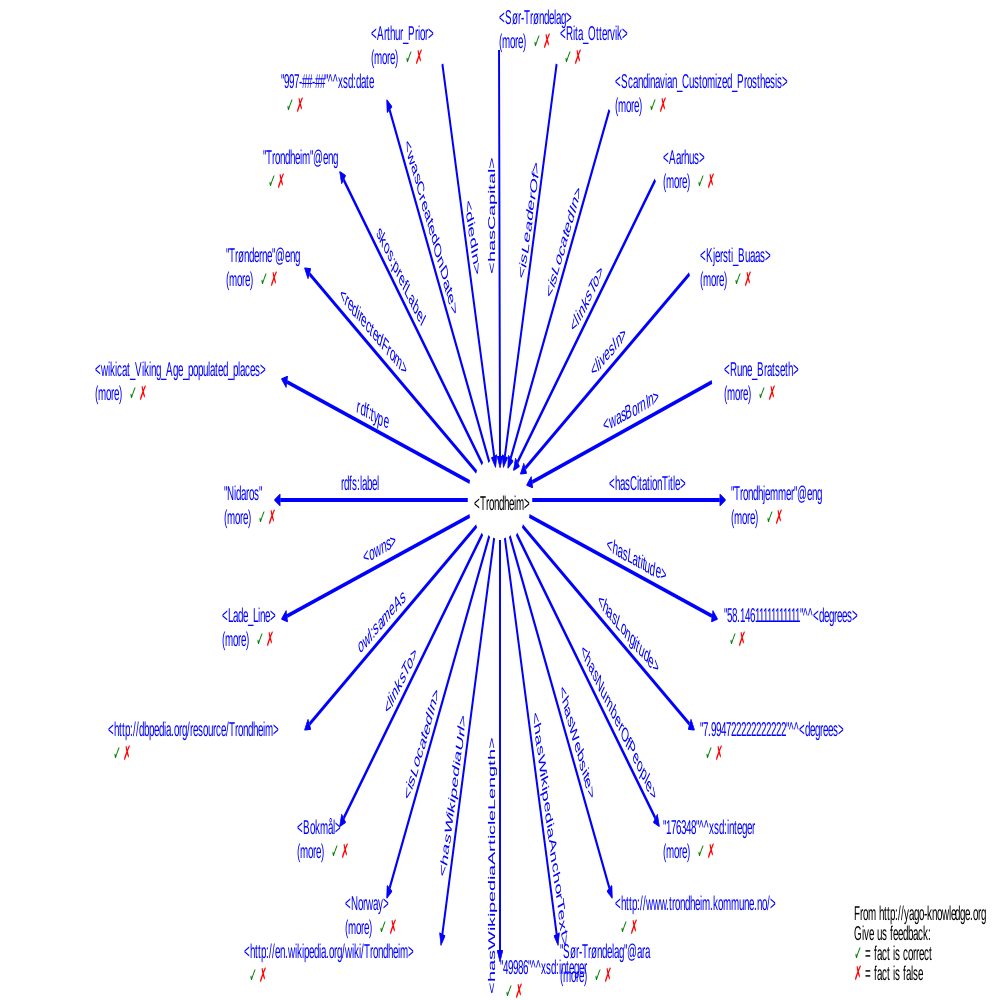
\includegraphics[scale=0.3]{figs/yago_trondheim.png}
 \caption{Trondheim as a subject in YAGO}
 \label{fig:Trondheim}
\end{figure}

\begin{figure}[t]
  \centering
  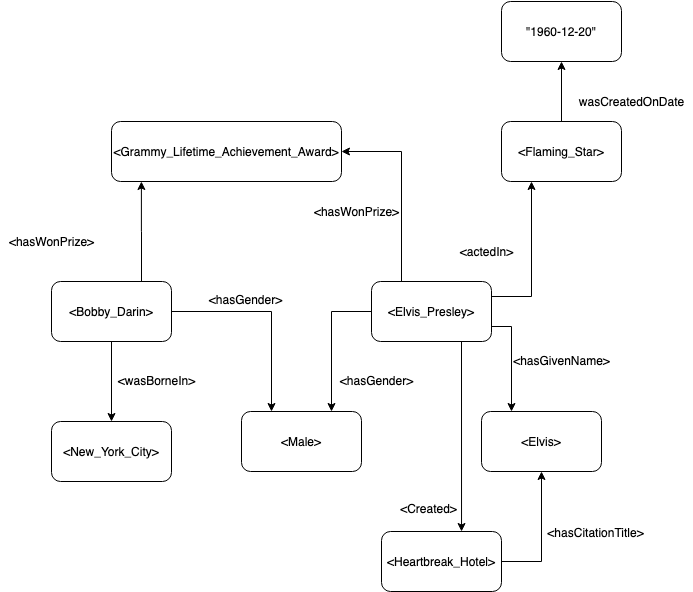
\includegraphics[scale=0.5]{figs/yagoExample.png}
 \caption{Connections in Yago around Elvis}
 \label{fig:Elvis}
\end{figure}

\section{Introducing Tables in the Report}

\glsresetall

%!TEX root = ../report.tex
\chapter{Architecture}
% OR: \chapter{Model}
\label{cha:architecture}

\section{Search}
\subsection{BFS search}
The most basic method of finding a match for keywords is using a breadth first search (BFS) \citep{blinks, Shi:2016:TRS:2882903.2882941}. For each keyword in the query the algorithm will find all vertices that contain the keyword. From that set of vertices the BFS search finds the first vertex that can connect all the vertices in the set. The vertex that connects the the rest of the set is the one that best fits the keywords in the search. There is however no guarantee that this set of vertices contains any spatial or temporal data. If this is the case, the search will continue until the a vertex containing spatial and temporal data is found. The first set of vertices containing all the keywords, a place, and time will be the best result using this search. The BFS search can however contain multiple times, or multiple places. To determine what time or what place best fits the query, a separate ranking algorithm can be used. BFS is also a time consuming algorithm and is used as a proof of concept and baseline in this thesis.

\begin{algorithm}[H]
    \caption{GetFullResultTree(p, t, Qt)}
    \SetAlgoLined
    \KwResult{Set containing all nodes with at least one keyword}
    Queue $\mathbf{Q}$ ADD(p)\; Threshold t\; Set n \;
    \While{$\mathbf{Q} \neq \emptyset$}{
        Clear(n)
        e=POP($\mathbf{Q}$)
        \If{GetDistance(e) > t}{
            continue\;
        }
        \ForEach{Term t $\in$ Qt}{
            \If{t $\in$ e}{
                p.AddMatchChild(e)\;
            }
        }
        \If{Qt $\subseteq$ e}{
            t = GetDistance(e)\;
        }
        n = GetNeighbors(e) \;
        $\mathbf{Q}$ ADD(n)\;
    }
\end{algorithm}

The first part of the search is to find a set of root nodes for sub-graphs. This is done by collecting all neighbors from the place queried. The neighbors can be connected by any predicate in the first developed algorithm, but as explain in \ref{pruning} this selecting specific predicates can greatly increase speed by limiting the amount of nodes traversed. The BFS algorithm described above is used for each of the possible roots of subgraphs, stopping when all keywords are matched, or the depth of the graph exceeds the three or exceeds the currently shallowest subgraph that has matched all keywords. The reason for limiting the depth of subgraphs is to ensure at least a partial hit within a reasonable time. Limiting the depth of subgraphs to the current shallowest subgraph is done because no a deeper graph cannot be a more accurate hit.

When traversing the graph and finding a match, a node object is created. This object is used to keep track of the pseudo hierarchy in the graph. All objects contain information on the depth of the node, matched query terms, and relation to parent and children, if any. In addition root objects contains a list of all query terms hit in the sub graph. If a child node is found within multiple subgraphs, a new object will be created representing the node for each subgraph. This creates some objects that are nearly identical, but with different relations and possible different depth.

When a node object is created, a document with tokens is created. This document is used to calculate score, and to match a node with the query words. A documnet is created from the last part of a Yago URI, after the last slash. Each URI si further split on each underscore, creating a list of words. 

\begin{algorithm}
\caption{minimum spanning graph}
\begin{algorithmic}[1]
\Procedure{minimum}{}
For each node in hits:\\
	for each minNode in min list:\\
		if node has same hits and higher depth than minNode:\\
			Break\\
		if node and minNode is equal in depth and hits:\\
			continue\\
		if node contains other words than minNode:\\
			add node\\
			remove potential common words from minNode\\
\EndProcedure
\end{algorithmic}
\end{algorithm}


After traversing the main graph we have found all subgraphs containing at least one query term. These subgraphs contain many nodes which hit the same terms. Before ranking the subgraphs the minimum spanning graph needs to be found. The minimum spanning tree is found using a greedy algorithm that iterates through all nodes in the subgraphs, then keeping the nodes containing the most terms, and lowest depth. The minimum tree will contain as many terms as possible, a term will only be found in one node, and the graph will be as shallow as possible.

- Find the minimum spanning tree for each of the root nodes containing the maximum amount of the query words.\\
- Rank based on 1. Query words hit 2. Nodes in the tree 3. depth of the tree\\
 % f(L(Tp), S(q, p)) = L(Tp) × S(q, p). \cite{Shi:2016:TRS:2882903.2882941} % Ranking formula 2
The final piece is to rank the minimum subgraphs. This is done using the nr. 2 formula found in \cite{Shi:2016:TRS:2882903.2882941}. 


\section{Pruning} \label{pruning}
When using the BFS search method, all possible spatial vertices close to the queried place will be explored. This is expensive and many of the vertices will be irrelevant. Pruning the potential place vertices will reduce the amount of subgraphs traversed, and will in turn reduce the overall time used to find results for the query.

\subsection{Predicate pruning}
When traversing the graph a lot of unnecessary predicates are followed, resulting in many extra nodes added to the search. Specifying a set of predicates that contain the relevant information can greatly increase the speed of the algorithm, and also keep the memory requirements a lot lower. When selecting predicates for traversal the information expected from the search should be the top priority. Because of this, all predicates that may contain spatial or temporal data should be kept.

When using the entirety of the Yago data set, most nodes are highly connected. Many of the links in the graph are from predicates such as ``linksTo'' or ``redirectedFrom''. These predicates creates a highly connected graph, and ensures a hit within a few nodes of the start. The same predicates will also often add the same nodes multiple times, create circular graphs, and take up unnecessary CPU power and memory.

When pruning predicates there are two methods that are possible to implement. The first will remove the predicates that contain little or no new information, such as ``linksTo'' or ``redirectedFrom'' mentioned above. This will still keep the graph connected, and keeps the predicates containing more useful information.

An other method of pruning is to create a list of predicates to be followed. This can drastically reduce the connections in the graph, but the results will only contain information relevant to the query. When preselecting predicates there is a much greater chance of not finding a match for a query. In addition a lot of metadata could be lost, if the metadata predicates are not added to the list of predicate to be explored.

\subsection{Unqualified place pruning}
For any spatial search, a lot of places will be found. The graph also contains information on the relationship between places. To find the best possible matches for a spatial query, only places of a higher resolution should be chosen. This means that places of similar or smaller expanse should be allows to be queried, e.g. a query of Boston can return the entirety of Boston, close to Boston, or within Boston. Massachusetts has multiple predicates linking it to Boston, but should not be queried because the information returned would be less detailed than what is queried. 

\subsection{Bounding}
When selecting places or times for a query, the boundaries should be set so that they encompass the entirety of the queried time and or place.

\glsresetall


%!TEX root = ../report.tex
\chapter{Experiments and Results}
\label{cha:Experiments}

\section{Experimental Plan}
\label{sec:experimentalPlan}
The goal of the experiments is to gather data for comparison of search methods. when comparing search methods, speed and accuracy will be the metrics used. Three methods for searching is used, one following all gathering all objects connected to an input subject, regardless of the predicate. One method following Yago predicates leading directly to a Yago URI. And the final method will follow the same predicates as the second, and will also add a condition where all nodes must match at least one query word.

\subsection{Time}
When timing the search, two different times will be measured, time for each query, and time for each root node. In addition to these, avg. nodes visited for each root will also be used. Taking the average of these over a large input set should generate an appropriate result. Both time metrics measure how fast results are found, so the results should be similar as long as the input data does not contain a high number of highly connected nodes.

The timing of the algorithm should be the same as any breath first search, $\Theta(\mathsf{V} + \mathsf{E})$ so that the best case is visiting only the first vertex, and the worst case is traversing the entire graph.


\subsection{Scoring and ranking}
Each query is given a score. This score will be used to see how pruning, and difference in predicates can lead to differences in the result tree. Two metrics for accuracy will be used, avg. accuracy for each result and avg. highest accuracy for each query.

\subsubsection{BFS}

\subsubsection{BFS with pruning}

% -------------------------------------------------------------------- %
\section{Experimental Setup}
\label{sec:experimentalSetup}

\section{Data set}
When selecting a data set an important feature was accurate spatial and temporal data. For this Yago was selected. Yago allows for download of subsets of data, and contains all the necessary data. The high accuracy in Yago was also a benefit of this data set. From Yago, the data selected was the entire Yago taxonomy, the entire Yago core, and from Genomes the sets GeonamesOnlyData, GeonamesClassIds, GeonamesGlosses, GeonamesTypes, and GeonamesClasses were selected. These sets makes it possible to build a complete graph of the entities in Yago, but keeps the disk usage as low as possible.\\

- Short description of each of the parts\\
- preprocessing: replace non-unicode chars, replacing space with underscore in URIs, terminate triplet where missing termination, remove double quotes in URIs, remove backslash unless legal escape sequence\\
- tdbloader for persistent queryable storage\\
- Structure of graph? Here or in Yago description?\\
% awk -F ' ' '{a[$1] += $2} END{for (i in a) print i, a[i]}' topMiddle100stemmed.txt | sort -k 2 -n > topMiddle.txt


\section{Queries}
When selecting the keywords used in queries, a semi random selection method was used at first. This method created three pools of words, rare words (less than 1000 occurrences) uncommon words (less than 100 000 occurrences) and common words (more than 100 000 occurrences). The three pools where created by stemming all words, then counting occurrences. From each pool of words, a set of 100 where randomly selected, and from those 100, 10 where selected manually to ensure a range of occurrences, and to ensure no stop words, misspelled words or other errors were in the final set of keywords.\\

A second set of words were also chosen to ensure a larger hit rate. This set was a random selection of 20 words from the top 150 words. From the 20 random words 10 where manually selected, the 150 word number was selected based on Zipfs law \cite{zipf}.\\

When selecting places for spatial queries, a set of 20 random places were selected from the YagoGeonamesOnlyData set, and from that set, 5 were chosen manually for the final set. In the final set, three places where added manually, Oslo, London, and New York City were added to ensure variation in placement and node connections.\\

Generating random queries can create results that will not have any hits.\\
Find a good method of creating queries.\\

\section{Pruning}
A simple method to improve performance when searching in large data sets is to remove data that is unnecessary to search.

\subsection{Predicate pruning}
Predicate pruning is the process of eliminating predicates from the search. The taxonomy of Yago creates assigns predicates to one or more group or class. By selecting specific groups or classes it is possible to follow the types of data searched for, while eliminating a lot of other data. When pruning based on classes or groups the type of data returned must be known beforehand, to ensure that no possible hits is overlooked.\\

Another possible method for pruning is to specify the exact predicates to follow. This will remove a lot of data, but is possibility when searching for something specific. This will also greatly increase the speed of the search, and reduce the memory usage for the search. 


% -------------------------------------------------------------------- %
\section{Experimental Results}
\label{sec:experimentalResults}

\section{BFS search}
BFS search without any pruning and search depth of 3 were unable to finish due to memory constraints and taking too long. Search with a depth of 2 may finish, depending on on the connectedness of the nodes discovered, and the amount of root nodes found in the search.

\subsection{Time}
When running the query, two sets are displayed, one with mostly random input data, and one with more closely selected data.

Because most of the randomly selected places had few possible root nodes, the table contains only the manually selected.

- time/query \\
- time/root \\
- roots found/ query \\

- accuracy/ result\\
- avg highest accuracy/ query\\

\begin{tikzpicture}
\begin{axis}[
	title={Avg. time/ query in ms},
	every axis plot post/.style={/pgf/number format/fixed},
	symbolic x coords={"No pruning", "No pruning 1 depth", "Pruning"},
	visualization depends on=rawy\as\rawy, % Save the unclipped values
	nodes near coords={\pgfmathprintnumber{\rawy}},
    xtick=data]
    \addplot[ybar,fill=blue] coordinates {("No pruning",159709.6486) ("No pruning 1 depth",14714.6216) ("Pruning",390.5810)};
\end{axis}
\end{tikzpicture}
%
\begin{tikzpicture}
\begin{axis}[
	title={Avg. time/ root in ms},
	every axis plot post/.style={/pgf/number format/fixed},
	symbolic x coords={"No pruning", "No pruning 1 depth", "Pruning"},
	visualization depends on=rawy\as\rawy, % Save the unclipped values
	nodes near coords={\pgfmathprintnumber{\rawy}},
    xtick=data]
    \addplot[ybar,fill=blue] coordinates {("No pruning",104.08202) ("No pruning 1 depth",9.58944) ("Pruning",0.2545398)};
\end{axis}
\end{tikzpicture}


\subsection{Accuracy}

\begin{tikzpicture}
\begin{axis}[
	title={Avg. nodes/ root},
	every axis plot post/.style={/pgf/number format/fixed},
	symbolic x coords={"No pruning", "No pruning 1 depth", "Pruning"},
	visualization depends on=rawy\as\rawy, % Save the unclipped values
	nodes near coords={\pgfmathprintnumber{\rawy}},
    xtick=data]
    \addplot[ybar,fill=blue] coordinates {("No pruning",3733.2554) ("No pruning 1 depth",263.2276) ("Pruning",1.0220)};
\end{axis}
\end{tikzpicture}
%
\begin{tikzpicture}
\begin{axis}[
	title={Avg. accuracy/ hit},
	every axis plot post/.style={/pgf/number format/fixed},
	symbolic x coords={"No pruning", "No pruning 1 depth", "Pruning"},
	visualization depends on=rawy\as\rawy, % Save the unclipped values
	nodes near coords={\pgfmathprintnumber{\rawy}},
    xtick=data]
    \addplot[ybar,fill=blue] coordinates {("No pruning",0.08353006) ("No pruning 1 depth",0.2654491) ("Pruning",0.26523)};
\end{axis}
\end{tikzpicture}
%
\begin{tikzpicture}
\begin{axis}[
	title={Avg. overall accuracy},
	every axis plot post/.style={/pgf/number format/fixed},
	symbolic x coords={"No pruning", "No pruning 1 depth", "Pruning"},
	visualization depends on=rawy\as\rawy, % Save the unclipped values
	nodes near coords={\pgfmathprintnumber{\rawy}},
    xtick=data]
    \addplot[ybar,fill=blue] coordinates {("No pruning",0.01064373) ("No pruning 1 depth",0.0039040070) ("Pruning",0.00390785)};
\end{axis}
\end{tikzpicture}
%
\begin{tikzpicture}
\begin{axis}[
	title={Avg. top accuracy/ query},
	every axis plot post/.style={/pgf/number format/fixed},
	symbolic x coords={"No pruning", "No pruning 1 depth", "Pruning"},
	visualization depends on=rawy\as\rawy, % Save the unclipped values
	nodes near coords={\pgfmathprintnumber{\rawy}},
    xtick=data]
    \addplot[ybar,fill=blue] coordinates {("No pruning",0.2648955) ("No pruning 1 depth",0.245495) ("Pruning",0.24549)};
\end{axis}
\end{tikzpicture}

\glsresetall

%!TEX root = ../report.tex
\chapter{Discussion and limitations}
\label{cha:Discussion}
In this chapter the methods implemented, and how these methods can be changed or extended to improve speed and accuracy are explored.

% 
% Du diskuterer dine resultater, men jeg kan ikke se at du sammenlikner dine resultater med hva andre har publisert. Det er viktig å  sammenlikne resultater ed hva andre har funnet. Det kan styrke dine resultater.
% Kan du få fram tydeligere hva som er nytt i dine resultater. Novelty????
% 
\section{Discussion}
\label{sec:Discussion}
% \item[Research question 1] {\em How can spatiotemporal data be integrated into exiting keyword query methods for RDF data.}
Using traditional methods for graph traversal it is possible to implement keyword search on RDF graphs. One such method is the use of BFS to find a minimum spanning subgraph containing the query words. Using spatial vertices as a root for the subgraph, creating a minimum spanning tree, it is possible to retrieve spatial data from such a keyword search. The same method is used when searching for spatial data as with other keyword searches, with the key difference being to root the BFS in a spatial vertex.

This BFS method can be implemented with a temporal dimension instead of spatial. When changing the data type of the root from spatial to temporal, the traversal method stays the same, but the root used is matched with temporal input instead of spatial input. The result tree for a temporal search can be ranked using the same methods as used for spatial search.

Combining spatial and temporal data makes spatiotemporal search possible. These searches will be rooted in a vertex containing spatial and temporal data matching the input, as defined by ``Spatiotemporal root'' in chapter \ref{rootST}. Because the root needs to contain both the spatial and the temporal input, the subset of vertices containing this will be small. This makes spatiotemporal searches quick to execute, but the accuracy and hit rate will be low. A method that could be implemented to increase the hit rate of these searches would be to change the criteria for one of the two dimensions. The search could be rooted in either space or time, and then look for the other dimension as a special case while traversing.

\subsection{Spatial and temporal vertices as special cases}
Spatiotemporal searches rooted only in time could be accomplished by discarding all result trees that are does not contain a vertex inside the queried location. To discover vertices inside a location the ``isLocatedIn'' predicate would be followed. Using this predicate to move upwards in the hierarchy the predicate creates while looking for the queried location will determine if the discovered vertex is located inside the queried location. A maximum distance of three should be used when following this predicate, as this will traverse the hierarchy up to at least country level, and possibly up to the earth vertex. Since we are looking for a specific vertex, and only looking at the vertices above in the hierarchy this will not add more than three extra visited vertices for each vertex connected with the isLocatedIn predicate. This will not increase the time used by any significant margin compared to the regular temporal search but will increase the hit rate of spatiotemporal search.

Rooting spatiotemporal search in a spatial vertex and treating the temporal dimension as a special case can be done with three different methods. Two of the methods is accomplished by looking at the predicate, and the third checks the type of literals. When using the predicate to determine if the connected vertex is temporal, the predicate can either be checked against a predetermined list of temporal predicates, or the range of valid values can be checked. Because predicates can also be treated as vertices the range can be determined by checking if the predicate have another predicate called ``rdfs:range'' connected to it. The ``rdfs:range'' predicate will have a literal on the other end. Checking if the range is ``xsd:date'' or ``xsd:dateTime'' will determine if the predicate is temporal. The final method, checks if the type of the literal is ``xsd:date'' or ``xsd:dateTime''. Since all literals have a type as part of the vertex, this is done by reading directly from the literal. Checking the predicate would add an extra traversal to each predicate connected to a vertex since the rdfs:range is treated as any other vertex. Using a predetermined list requires more knowledge of the data set and adds some small overhead. Checking the type of the objects is the fastest since this would not require any extra traversal and carries little overhead. This would not require any extra knowledge about the data set, assuming that no extra user added temporal types are created for the graph.

\subsection{Reduction of vertices and edges}
Since the number of vertices visited is the factor most correlated to time used for a search, reducing the amount of vertices visited will also reduce the time used for a search. To reduce the number of vertices, a possibility is to reduce the predicates followed. Following predicates based on type can be used to create search methods that will only follow specific predicates. This can be accomplished using natural language processing, similar to what is done in \cite{4812421,aqualog}. A less sophisticated method would be to allow for the selection of categories to be searched, then using the selected categories to extract all predicates that are connected. Because the predicates have types and properties, running a query to find all connected predicates to a category would not add more than two extra traversals, one for type, and one for property. Such a category would contain a set of types and properties that would be used to find predicates. This would make it easy to add new predicates, without having to rework the search. The same categories can be used for natural language processing, but then the query have to be preprocessed to find the categories that should be included. A downside of removing predicates, is the possibility of missing some results, and decreasing the accuracy.

Reduction of root vertices is also a method that can be implemented to increase the speed of a search. To be able to reduce the roots while maintaining accuracy, using more sophisticated natural language processing is an option. Implementing a system for inferring structure from the keywords, like that used in \cite{Elbassuoni:2011:KSO:2063576.2063615} would make it possible to find connections where the object and predicate is related to the query. Using the taxonomy from YAGO, this is possible to implement.

\subsection{Indexing and natural language processing}
It is possible to index the vertices in the graph, so that they can be searched using full text search. If all vertices are tokenized and indexed so that all vertices containing a keyword can be retrieved, this can be combined with the roots for temporal, spatial or spatiotemporal searches. Using SPARQL it is possible to find paths between two vertices using ``property paths''. From this, the shortest paths between a root and keyword vertex can be determined, and finally the roots can be ranked. This will guarantee hits for all roots, but it could be painfully slow, depending on the input keywords. Using the keyword ``south'' as an example, this keyword has 2\,798\,973 hits in the YAGO data used for the experiments in this thesis. Combining this with the average number of temporal roots from section \ref{sec:experimentalResults}, 192, this search would have to query and rank 537\,395\,904 paths, just for one keyword. Using such an index would require more than just the shortest path.

Using an index for keywords to find shortest paths without exploring the entire graph will find the best result for a given keyword. Depending on how it is implemented, it might not find the best solution for vertices containing multiple keywords. This is because a vertex containing more than one keyword at a greater distance may score higher than multiple vertices containing one keyword each at a shorter distance. The score would depend on the number of keywords in a single vertex, and the difference in depth. If even a single vertex is found at the same depth as the multi-keyword vertex, the result tree with the fewest vertices will score better.

\section{limitations}
Some temporal vertices in YAGO use a so called ``wildcard date''. These dates contain a ``\#'' symbol for parts of the date, making it impossible to directly query such dates when selecting roots. This means that the temporal search has some possible vertices missing from the set of root vertices used when traversing the graph. This could have been remedied by creating two new temporal vertices for such dates, one start date indicating the lowest possible value a wildcard date could have, and an end date indicating the highest possible value a wildcard could have.

When searching spatiotemporal data, the wildcards have been used. This was done by adding logic comparing the wildcards found connected to spatial vertices to the date range in the search. By doing this, the spatiotemporal search should be more accurate, and should retrieve some vertices that a regular temporal search would not retrieve.

Because of the large number of vertices discovered during a search, memory would run out on traversal with high distance from root. This could be solved by writing to disk, but would be slow, and since the search already reads from disk to load vertices, this would have a significant impact on search time. When testing without any form of pruning, the computer would run out of memory. Because of this, no results are gathered from a method following all edges of each vertex. Following all edges on each vertex would also lead to highly connected category vertices being discovered, resulting in artificially high hit rates for such searches.
%!TEX root = ../report.tex
\chapter{Conclusion and future work}
\label{cha:Conclusion}
This thesis have explored search methods for RDF graphs, finding methods for spatial, temporal, and spatiotemporal search. By building on existing keyword search methods, a new method for spatiotemporal search have been introduced and evaluated. From the evaluation further improvements have been proposed.

\section{Contributions}
\label{sec:Contributions}
This thesis had the goal to research methods for keyword searches on large spatiotemporal RDF graphs. This was broken down into three research questions.

\begin{description}
    \item[Research question 1] {\em How can spatiotemporal data be integrated into existing keyword query methods for RDF data?}
\end{description}
In the chapter \ref{cha:related_work} previous methods used for keyword searches on RDF graphs was investigated. Using methods from other research, spatiotemporal keyword search have been implemented. The effectiveness of the search can be further improved, and by treating one of the two dimensions as special cases, the accuracy of spatiotemporal searches can be further improved.

\begin{description}
    \item[Research question 2] {\em What methods can be used to achieve greater speed and accuracy for searches on RDF data?}
\end{description}
This thesis looked at the parameters of a search that could increase speed, and decrease accuracy. When increasing speed, the main goal should be to reduce the amount of vertices visited during traversal. Reducing the edges followed is one of the primary methods to accomplish this. By pre-processing the query a structure can be created from the keywords that can be used to create more effective queries.

\begin{description}
    \item[Research question 3] {\em How do spatial and temporal RDF query methods differ from other query methods?}
\end{description}
Using a BFS for traversing the graph, a spatiotemporal search does not need to differ from spatial or temporal search. Spatial and temporal searches differ from regular keyword searches by rooting the subgraph in a vertex containing data for the queried dimension. When selecting the roots used as starting points for the search, a spatiotemporal search needs to find roots that fall into both the spatial dimensions of the search, and the temporal. This makes the total set of roots used for a spatiotemporal search less than if the search was done just on one dimension.

\section{Future work}
\label{sec:futureWork}
Further research into spatial, temporal, and spatiotemporal keyword search on RDF graphs can make the technology more accessible. Exploring search methods implementing natural language processing for pre-processing of queries, similar to \cite{aqualog} could improve accuracy of search. Relying more on the ontology to infer meaning from a keyword search can also make searching RDF graphs faster and more accurate.

Because each search is rooted in one specific root, and traverse the graph from that root, parallelizing the search should be researched. Running multiple traversals at the same time would not affect any of the other traversals result trees but would make it possible to execute a search faster. This would not affect the accuracy, and can be implemented on many of the existing search methods for RDF graphs.

Finally, treating spatial or temporal data as a special case while traversing the graph, as discussed in chapter \ref{cha:Discussion} could be considered a continuation of this thesis. Testing these search methods can give insight into how spatiotemporal searches on RDF graphs can be further improved.

%%%%%%%%%%%%%%%%%%%%%%%%%%%%%%%%%%%%%%%%%%%%%%%%%%%%%
\backmatter

\addcontentsline{toc}{chapter}{Bibliography}
\bibliographystyle{plainnat}
\bibliography{bib/bibliography}
% alternative, if using biber as backend
% \printbibliography

%!TEX root = ../report.tex
\appendix

\chapter{Appendices}
\label{cha:appendices}
\section{Spatial search source code}
Source code for spatial search can be found in the spatial folder in the source code zip file. The source code is also available on GitHub at \url{https://github.com/MrHanSan/master_thesis/tree/spatial/code/st-rdf}

\section{Temporal search source code}
Source code for temporal search can be found in the temporal folder in the source code zip file. The source code is also available on GitHub at \url{https://github.com/MrHanSan/master_thesis/tree/temporal/code/st-rdf}

\section{Spatiotemporal search source code}
Source code for spatiotemporal search can be found in the spatiotemporal folder in the source code zip file. The source code is also available on GitHub at \url{https://github.com/MrHanSan/master_thesis/tree/spatiotemporal/code/st-rdf}


\end{document}
